\documentclass[11pt,a4paper]{article}

\usepackage[frenchb]{babel}
\usepackage[autolanguage]{numprint}
\usepackage[margin=2cm]{geometry}
\usepackage[utf8]{inputenc}
\usepackage[T1]{fontenc}
\usepackage{hyperref}
\usepackage{listings}
\usepackage{gensymb}
\usepackage{graphicx}
\usepackage{pdflscape}
\graphicspath{ {images/} }

\begin{document}
	
	\title{
		Compte-rendu du TP C++ 4\\
		Conception
	}
	\author{
		Arnaud Favier\\
		\and
		Marc Gagné
	}
	\date{Février 2016}
	\maketitle
	
	\section*{Préambule}
	Nous avons fait le choix de séparer le programme en trois grandes parties, séparées mais dépendantes l'une de l'autre :
	\begin{itemize}
		\item L'interface avec l'utilisateur, qui gère les entrées et sorties et contrôle les deux autres parties,
		\item Le gestionnaire d'historique, responsable de la mémorisation des actions de l'utilisateur, afin de pouvoir les défaire ou les refaire,
		\item Le modèle géométrique, indépendant du reste du programme, qui décrit les différentes figures et leur règles.
	\end{itemize}
	Les différentes classes réalisant ces trois parties sont présentées ci-dessous, avec leurs attributs et méthodes principales.
	
	\section{Interface utilisateur}
	L'interface fait le lien entre l'utilisateur et le modèle, en gérant les ajouts, suppressions et modifications des différentes figures, en enregistrant les modifications effectuées dans le gestionnaire d'historique.
	
	\subsection{Editor}
	Cette classe fonctionne en permanence grâce à sa méthode \texttt{run}, qui tourne tant que le programme est actif : la méthode lit l'entrée standard, attendant que l'utilisateur fournisse des commandes ; ces commandes sont ensuite interprétées et retransmises au reste du programme. La classe est responsable de la validation des commandes (vérification que la commande existe, qu'elle fournit le bon nombre d'arguments…) et indique à l'utilisateur lorsqu'un problème survient.
	
	\subsection{\texttt{Canvas}}
	La classe “principale” du programme, \texttt{Canvas} lie toutes les parties différentes du programme ensemble. Les commandes de l'utilisateur, lues par Editor, sont concrètement exécutées ici ; si la commande modifie le modèle, le \texttt{Canvas} fournit toutes les informations nécessaires à l'instance de \texttt{HistoryManager} stockée dans \texttt{historyMgr} pour qu'elle puisse défaire ou refaire cette commande à l'avenir.
	
	Le \texttt{Canvas} gère la collection de toutes les figures géométriques qui ont été crées dans figures, une map associant les noms des figures à des pointeurs vers des figures ; cette collection stocke l'ensemble du mo. Les figures sont ajoutées à travers les méthodes \texttt{addSegment}, \texttt{addRectangle}, \texttt{addConvexPolygon}, \texttt{addUnion} et \texttt{addIntersection}, qui vérifient d'abord qu'une figure avec ce nom n'existe pas encore, avant de la construire puis de l'ajouter à la collection. Le gestionnaire d'historique est également informé de l'ajout, en lui fournissant une copie de la figure créée. Ces figures peuvent ensuite être déplacées avec la méthode \texttt{move} (qui donne le nom de la figure déplacée et son vecteur de déplacement à \texttt{HistoryManager}) ou supprimée avec la méthode \texttt{deleteFigures} (qui fournit au gestionnaire d'historique une copie de chaque figure au moment de sa suppression, pour qu'elle puisse être recréée si l'utilisateur le désire). Si l'utilisateur veut tout supprimer et réinitialiser le \texttt{Canvas} (mais pas son historique), la méthode \texttt{clear} peut être utilisée (ce qui crée encore une entrée dans le gestionnaire d'historique, afin de taut restaurer d'un coup).
	
	L'état du \texttt{Canvas} peut ensuite être visualisé à travers les méthodes \texttt{list} (qui affiche une liste de toutes les figures crées à l'écran, dans le même format que les fichiers d'enregistrement) et contains (qui vérifie si une figure contient un point). Comme ni l'une ni l'autre ne modifie l'état du modèle, le gestionnaire d'historique n'est pas affecté par l'appel de ces méthodes.
	Pour assurer la persistence du modèle, les commandes \texttt{save} et \texttt{load} peuvent être utilisées pour enregistrer et restaurer un modèle, respectivement (la commande load ajoute une entrée dans le gestionnaire d'historique ; si un \texttt{undo} est effectuée sur une opération de chargement, toutes les figures qui avaient été créées sont supprimées). Les fichiers produits consistent en une liste de toutes les figures, identifiées par leur nom et un caractère (\texttt{S} pour un segment, \texttt{R} pour un rectangle, \texttt{C} pour un polygone convexe, \texttt{U} pour une union et \texttt{I} pour une intersection), suivis des paramètres nécessaires à la construction de la figure (dans une liste encadrée par \texttt{[} et \texttt{]}).
	
	Finalement, les commandes \texttt{undo} et \texttt{redo} permettent d'avancer ou de reculer dans l'historique. Elles renvoient une erreur lorsque le début ou la fin (respectivement) de l'historique est atteint.
	
	\section{Gestionnaire d'historique}
	Chaque opération effectuée dans le \texttt{Canvas} qui modifie le modèle géométrique est sockée dans le gestionnaire d'historique, qui permet de défaire et de refaire ces opérations, du lancement de l'application à sa ferméture.
	
	\subsection{\texttt{HistoryManager}}
	Cette classe gère la liste d'événements qui ont modifié le modèle. Les événements sont stockés dans le vecteur history, et la position actuelle dans cet historique est stockée dans current : cette variable est incrémentée lorsqu'une opération est effectuée (soit lorsque c'est la première fois qu'elle est effectuée, soit lorsqu'elle est refaite après avoir été défaite), et décrémentée lorsqu'une opération est défaite. Ceci est possible grâce aux méthodes \texttt{addEntry} (à appeler lorsqu'une opération qui a modifié le modèle a été effectuée), \texttt{undo} et \texttt{redo} (pour défaire et refaire des opérations).
	
	\subsection{\texttt{HistoryEntry}}
	Les opérations effectuées par l'utilisateur sont stockées sous forme d'instances sous-classées de \texttt{HistoryEntry}. L'ensemble des opérations possibles a été divisé en trois catégories, représentées par trois sous-classes :
	\begin{itemize}
		\item \texttt{FigureEntry} : représente la création ou la destruction d'une figure. La figure à recréer, si nécessaire, est fournie dans figure, son nom est dans name, et le type d'opération est spécifié par le booléen deleted. Cette dernière variable détermine si la figure sera recrée ou supprimée lorsque cette opération est défaite ou refaite.
		\item \texttt{MoveEntry} : représente le déplacement d'une figure. Le nom de la figure déplacé est stocké dans name, et le vecteur de déplacement est enregistré dans delta.
		\item \texttt{GroupEntry} : cette opération ne représente pas une opération en particulier, mais permet de regrouper plusieurs autres en une seule, ce qui est utile pour défaire ou refaire plusieurs opérations d'un seul coup (par exemple, dans le cas du chargement d'un fichier).
	\end{itemize}
	Ces entrés sont générées par \texttt{Canvas} et transmises à \texttt{HistoryManager}, qui devient responsable de leur gestion.
	
	\section{Modèle géométrique}
	Le modèle prend la forme d'un ensemble de types de figures géométriques différentes regroupées ensemble. Toutes les figures dérivent de la classe de base \texttt{Figure}.
	
	\subsection{Figure}
	La classe Figure est une classe abstraite, contenant une série de caractères permettant l'identification du type de ses filles (car il n'y a pas de mécanisme d'introspection en C++) via l'appel à la méthode \texttt{getType}, définie virtuelle pure et qui retourne le caractère correspondant. Ces caractères sont définis statiques et constants.
	
	Cette classe ne comporte pas d'attributs, mais contient un ensemble de méthodes. La méthode \texttt{as} retourne l'instance courante (\texttt{this}) casté suivant le type demandé dans l'appel. Attention donc à bien appeler la méthode avec le bon type (déterminé suivant le caractère d'identification précédent) pour avoir un cast correct. La méthode \texttt{contains} est virtuelle pure et retourne un booléen suivant si la figure contient le point \texttt{Vector2D} passé en paramètre (\texttt{true}) ou non (\texttt{false}). Pour avoir une copie de la figure courante, la méthode \texttt{createCopy}, qui est virtuelle pure, est appelée et retourne un nouvel objet grâce au constructeur par copie de la classe fille, qui doit implémenter cette méthode. La méthode \texttt{move} est définie virtuelle pure, et déplace la figure d'une distance exprimée par un \texttt{Vector2D}, passée en paramètre. Enfin, la classe \texttt{Figure} surcharge les deux opérateurs \texttt{<<} et \texttt{>>} en les déclarant fonctions amies pour un affichage simplifié des figures filles.
	
	\subsection{\texttt{Polygon}}
	La classe \texttt{Polygon} hérite de \texttt{Figure} et définit les formes géométriques que l'on peut considérer comme étant un polygone. Le constructeur prend en paramètre un vecteur de points \texttt{Vector2D}, représentant la liste des points constituant le polygone, qui seront ensuite stockés en attribut de la classe.
	
	La méthode \texttt{move} est implémentée, et sera utilisée pour l'ensemble des classes filles. Deux méthodes sont aussi présentes : \texttt{serializePoints} qui écrit le vecteur de points du \texttt{Polygon} dans un stream au format de sortie défini dans le cahier des charges détaillé, pour ensuite l'afficher sur la console, ou l'enregistrer dans un fichier, et \texttt{unserializePoints}, qui fait l'inverse de la fonction précédente, à savoir peupler le vecteur de points du \texttt{Polygon} à partir d'un stream issu du chargement d'un fichier au format défini. Autrement la classe se charge simplement de réécrire les prototypes des méthodes virtuelles pures pour avoir un code plus compréhensible par la suite.	
	
	\subsubsection{\texttt{Segment}}
	Un \texttt{Segment} est composé de deux points \texttt{Vector2D} qui sont les deux extrémités du segment. La classe hérite de \texttt{Polygon}, et le constructeur prend les deux points qui seront passés comme liste en paramètre au constructeur de \texttt{polygon}.
	
	La méthode \texttt{contains} est définie, avec les opérations mathématiques du produit vectoriel dans un premier temps, puis du produit scalaire par la suite, pour déterminer l'appartenance ou non à un segment du point passé en paramètre. La méthode \texttt{createCopy} retourne un nouvel objet grâce au constructeur par copie (celui par défaut est utilisé), et \texttt{getType} renvoie le type attendu grâce au caractère défini dans la classe \texttt{Figure}. L'opérateur \texttt{<<} est surchargé, et appelle la méthode mère \texttt{serializePoints}, et l'opérateur \texttt{>>} fait appel à la méthode mère \texttt{unserializePoints} et retourne un nouveau segment avec les points qui viennent d'être initialisés.
	
	\subsubsection{\texttt{Rectangle}}
	Un rectangle est un polygone composé de deux points \texttt{Vector2D} qui sont le point haut gauche et le point bas droit du rectangle. La classe hérite donc de \texttt{Polygon}, et le constructeur prend les deux points qui seront passés comme liste en paramètre au constructeur de \texttt{Polygon}.
	
	La méthode \texttt{contains} est définie, et regarde si le point passé en paramètre se trouve dans les limites définies par les coordonnées des deux coins opposés du rectangle, pour déterminer l'appartenance ou non à ce dernier. La méthode \texttt{createCopy} retourne un nouvel objet grâce au constructeur par copie (celui par défaut est utilisé), et \texttt{getType} renvoie le type attendu grâce au caractère défini dans la classe \texttt{Figure}. L'opérateur \texttt{<<} est surchargé, et appelle la méthode mère \texttt{serializePoints}, et l'opérateur \texttt{>>} fait appel à la méthode mère \texttt{unserializePoints} et retourne un nouveau rectangle avec les points qui viennent d'être initialisés.
	
	\subsubsection{\texttt{ConvexPolygon}}
	Un polygone convexe est un polygone (donc hérite de la classe \texttt{Polygon}) composé d'une liste de points \texttt{Vector2D}. On rappelle que le polygone doit être convexe (angles inférieurs à 180\degree) et non croisé. Cela ne sera pas vérifié et dépend de la responsabilité de l'utilisateur. Le constructeur prend une liste (sous la forme d'un \texttt{vector}) de points \texttt{Vector2D} passée en paramètre au constructeur de \texttt{Polygon}.
	
	La méthode \texttt{contains} est définie, et regarde si le point passé en paramètre se trouve toujours du même côté que les côtés du polygone. Si le point est de l'autre côté, alors il est à l'extérieur du polygone. La méthode \texttt{createCopy} retourne un nouvel objet grâce au constructeur par copie (celui par défaut est utilisé), et \texttt{getType} renvoie le type attendu grâce au caractère défini dans la classe \texttt{Figure}. L'opérateur \texttt{<<} est surchargé, et appelle la méthode mère \texttt{serializePoints}, et l'opérateur \texttt{>>} est aussi surchargé et fait appel à la méthode mère \texttt{unserializePoints} et retourne un nouveau polygone avec les points qui viennent d'être initialisés.
	
	\subsection{\texttt{FigureGroup}}
	La classe \texttt{FigureGroup} hérite de \texttt{Figure} et est utilisée pour contenir un ensemble de sous-figures. C'est une classe abstraite qui contient une liste (\texttt{vector}) de \texttt{Figure}s en attribut, ainsi que des constructeurs par défaut, par copie, et la surcharge de l'opérateur \texttt{=}. La méthode \texttt{addFigure} permet d'ajouter une figure dans la liste d'ensemble des sous-figures. La méthode \texttt{move} est implémentée et appelle pour chaque sous-figure de la liste, leur propre méthode \texttt{move}. Pour la sérialisation, \texttt{serializeFigures} écrit la liste des figures dans un stream via l'appel à la surcharge de l'opérateur \texttt{<<} des figures, et \texttt{unserializeFigures} peuple la liste des figures à partir d'un stream, grâce à la surcharge de l'opérateur \texttt{>>}. Enfin, les prototypes de méthodes non implémentées de \texttt{Figure} sont recopiées pour les classes filles afin d'avoir un code lisible.
	
	\subsection{\texttt{Union}}
	Une union étant un ensemble de figures, la classe \texttt{Union} hérite de la classe \texttt{FigureGroup}, et le constructeur appelle celui de \texttt{FigureGroup} avec la liste des figures en paramètre. Un constructeur par copie est aussi présent. La méthode \texttt{contains} est implémentée, et appelle pour chaque figure de la liste sa méthode \texttt{contains}, avec le point passé en paramètre. Concernant \texttt{createCopy}, la méthode retourne une nouvelle instance d'union. Enfin, les opérateurs \texttt{<<} et \texttt{>>} sont surchargés, pour écrire une union dans un stream et en lire une nouvelle instance, respectivement. On fait alors appel à la méthode \texttt{serializeFigures} des figures de la liste.
	
	\subsection{\texttt{Intersection}}
	Une intersection étant un ensemble de figures, la classe \texttt{Intersection} hérite de la classe \texttt{FigureGroup}, et le constructeur appelle celui de \texttt{FigureGroup} avec la liste des figures en paramètre. Un constructeur par copie est aussi présent. La méthode \texttt{contains} est implémentée, et appelle pour chaque figure de la liste la méthode \texttt{contains} de la figure appropriée, avec le point passé en paramètre. Concernant \texttt{createCopy}, la méthode retourne une nouvelle instance d'intersection. Enfin, les opérateurs \texttt{<<} et \texttt{>>} sont surchargés, pour écrire une intersection dans un stream et en lire une nouvelle instance, respectivement. On fait alors appel à la méthode \texttt{serializeFigures} des figures de la liste.
	
	\begin{landscape}
		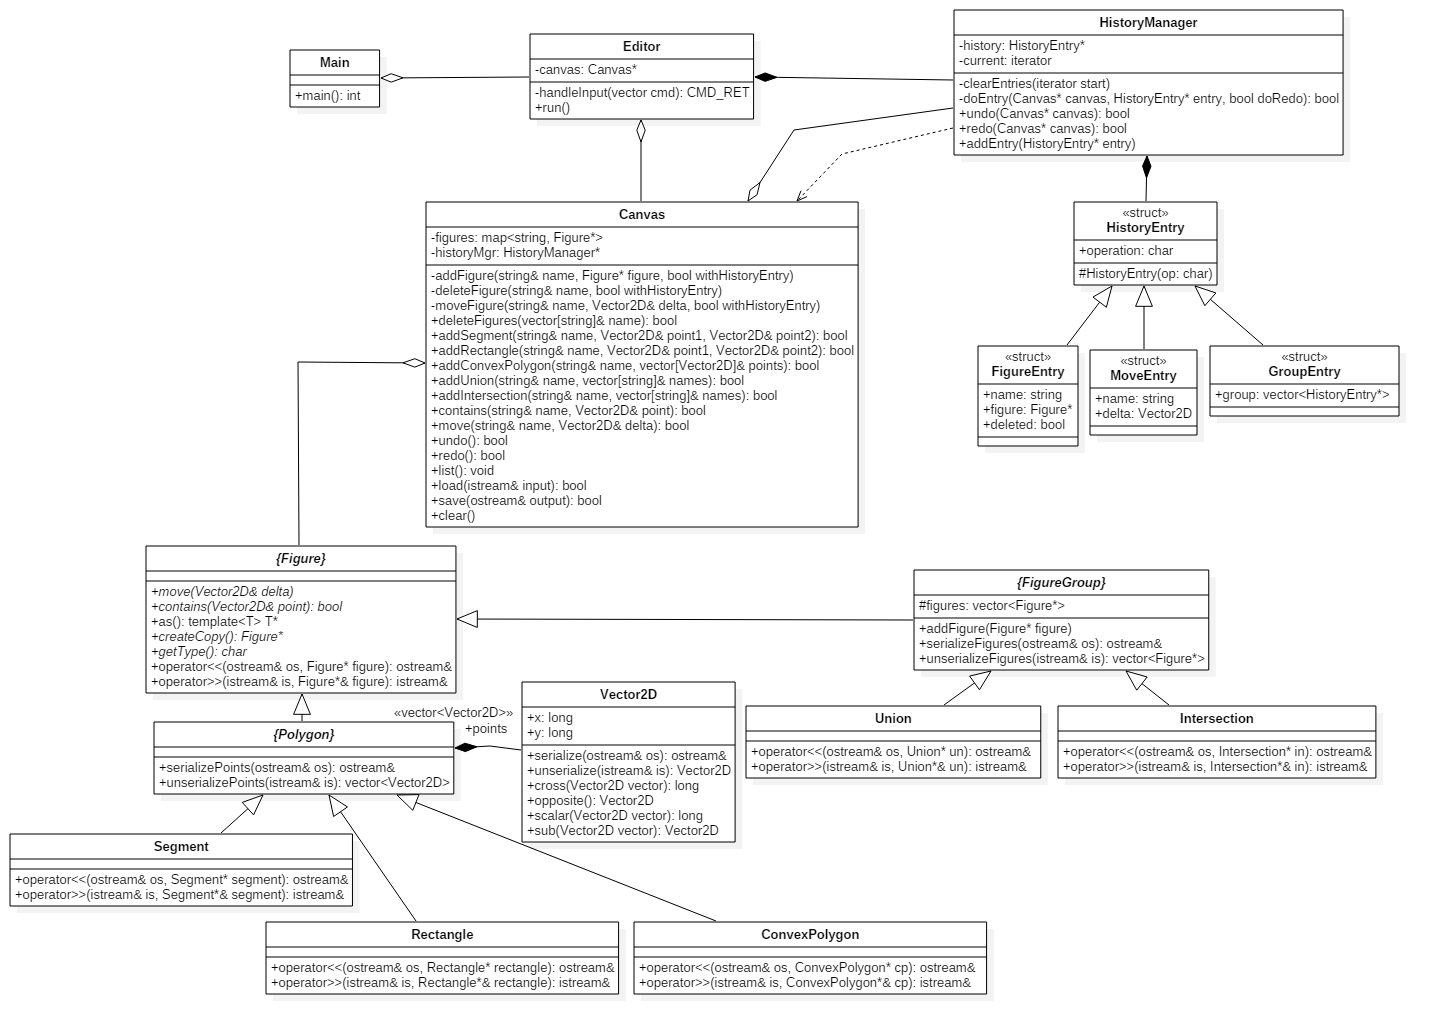
\includegraphics[height=\textwidth]{ClassDiagram}
	\end{landscape}
	
\end{document}